\documentclass{article}
\usepackage{amsmath}
\usepackage{mathtools}
\usepackage{tikz}
\usepackage{hyperref}
\usepackage{biblatex}
\usepackage{titling}
\usepackage{amsmath}
\usepackage{amssymb}
\usepackage{amsthm}
\usepackage{mathtools}
\usepackage{array}
\usepackage{tikz}
\usepackage{hyperref}
\usepackage{enumitem}
\usepackage{stmaryrd}
\usepackage{subcaption}
\usepackage{titling}

%%%% Title page commands %%%
\newcommand\email[1]{
    \href{mailto:#1}{\url{#1}}
}

% Takes: name, affiliation & email
\newcommand\authorblock[3]{
    #1\\
    \small{#2}\\
    \small{\email{#3}}
}

\newcommand\keywords[1]{
    \vspace{5mm}\noindent
    \small{\textbf{\textit{Keywords ---}} #1}
}

%%% Short-hands %%%
\newcommand\NN{\mathbb{N}}
\newcommand\ZZ{\mathbb{Z}}
\newcommand\RR{\mathbb{R}}
\newcommand\CC{\mathbb{C}}

%%% Theorem environments %%%
\newtheorem{thm}{Theorem}
\newtheorem{lemma}{Lemma}
\newtheorem{prop}{Proposition}
\theoremstyle{definition}
\newtheorem{defn}{Definition}

\date{\today}




\title{Simulating the Water Molecule using a Quantum Walk Algorithm}
\author{
    Floris van den Ende\\
    \small{Amsterdam University College}\\
    \small{\url{florisvdende@gmail.com}}\\
    \\
    \small{Supervisor}\\
    Jasper van Wezel\\
    \small{FNWI \& QuSoft}\\
    \small{\url{j.vanwezel@uva.nl}}\\ \\
    \small{Daily Supervisor}\\
    Joris Kattemolle\\
    \small{Qusoft}\\
    \small{\url{j.j.kattemolle@uva.nl}}
}

\begin{document}


\begin{titlepage}
    \newcommand{\HRule}{\rule{\linewidth}{0.5mm}}

	\center

	\HRule\\[0.4cm]

	{\huge\bfseries \thetitle\\[0.4cm]}

	\HRule\\[1.5cm]

	\begin{minipage}{0.45\textwidth}
		\begin{flushleft}
			\large
			\textit{Author}\\
            Floris van den Ende\\
            {\small Amsterdam University College}\\
            {\small\email{florisvdende@gmail.com}}
		\end{flushleft}
	\end{minipage}
	~
	\begin{minipage}{0.4\textwidth}
		\begin{flushright}
			\large
			\textit{Supervisor}\\
            Jasper van Wezel\\
            {\small{FNWI \& Qusoft}\\
            {\small{\url{j.vanwezel@uva.nl}}}}
		\end{flushright}
    \end{minipage}
    \\[1cm]
    \begin{minipage}[t]{0.45\textwidth}
		\begin{flushleft}
			\large
			\textit{Tutor}\\
            Forrest Bradbury\\
            {\small Amsterdam University College}\\
            {\small\email{f.bradbury@auc.nl}}
		\end{flushleft}
	\end{minipage}
	~
	\begin{minipage}[t]{0.4\textwidth}
		\begin{flushright}
			\large
			\textit{Daily Supervisor}\\
            Joris Kattemolle\\
            {\small Qusoft}\\
            {\small\email{J.J.Kattemolle@uva.nl}}
		\end{flushright}
	\end{minipage}
    \vfill\vfill\vfill

    {\large
        Major: Sciences\\[0.5cm]
        \thedate
          
           }

	\vfill

\end{titlepage}



\abstract{This capstone will build towards understanding complex chemical reactions with the usage of quantum computing, by examining the efficiency of the quantum walk algorithm proposed by Poulin et al. applied to the water molecule. This algorithm will be implemented into a circuit using Google's Cirq package and the ground state energy of the static water molecule will be retrieved. Ultimately, this capstone will compare the efficiency of aforementioned algorithm to several well-established other algorithms, of which the conclusions might be extrapolated to more complex chemical reactions. Quantum computing can help elucidate processes such as nitrogenase, where a greater understanding might lead to a severely reduced global energy output.}

\keywords{quantum computing, quantum walk, cirq, water molecule, quantum chemistry}

\section{Introduction}

\cite{bla}

3\% of the world's energy output is spent on making fertilizer (Citation). We currently rely on a highly outdated, energy intensive process requiring very large amounts of natural gas. There is an anaerobic bacteria however perfoming the very same process while requiring much less energy, utilizing nitrogen fixation with molecules such as FeMoCo. Traditional chemical analyses have not been able to give us an understanding on the details of this process, and as this molecule is highly complex, simulations using classical supercomputers are out of reach. Reiher et al. have shown that quantum computers are, even when taking in the substantial decoherence and error of today's algorithms, able to elucidate chemical processes such as nitrogen fixation in nitrogenase. Current research within quantum computing has not progressed quite enough to provide significant insight into nitrogenase, and this study aims to build towards understanding more complex chemical reactions with quantum computers by examining the efficiency of a quantum walk ground-energy algorithm on the water molecule. If the scientific community succeeds in elucidating nitrogenase, new and more efficient processes of creating fertilizer may be developed, significantly reducing the global carbon footprint.



\section{Research Context}

The most fundamental property of a static molecule is perhaps the energy of the  molecule in its ground state. Before any other significant conclusions can be drawn about a molecule, the ground state energy must be known and accurately measured. If the field of quantum computing wishes to contribute to the understanding of chemical processes, it must succeed in efficiently retrieving the eigenvalues and eigenstates of the Hamiltonian operator. The water molecule is simple enough for a classical computer to simulate, and the ground state energy can be determined with the Hartree-Fock method, allowing this thesis to find the accuracy of the results of the algorithm. The energy corresponding to the binding angle is portrayed in figure \ref{h2o}. 

\begin{figure}[htbp]
    \centering
    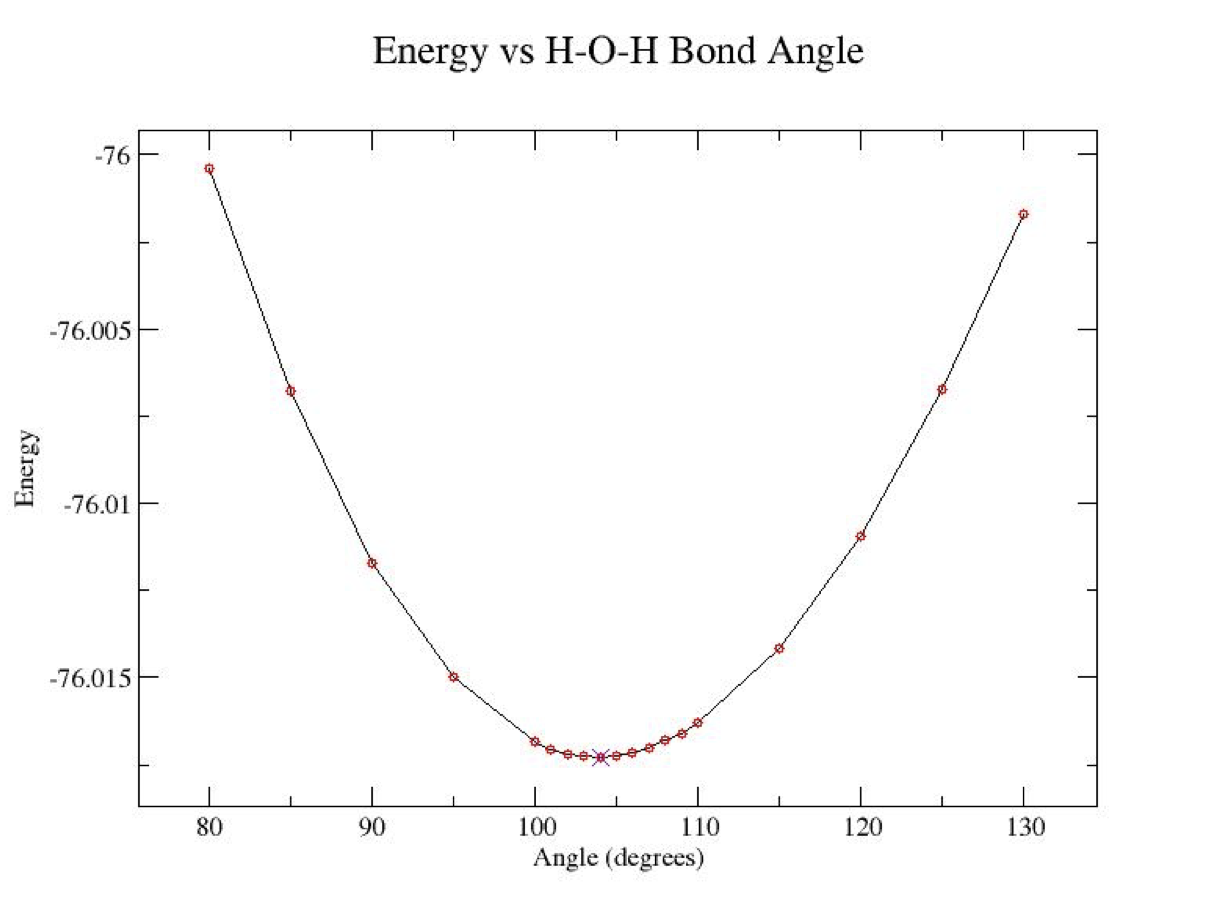
\includegraphics[scale=0.4]{h2oenergy.png}
    \caption{Energy of the H2O molecule, determined by the Hartree-Fock method (source).}
    \label{h2o}
\end{figure}

The second quantized Hamiltonian of the static water molecule generally has the form:

$$
H=\sum_{i, j=1}^{12} h_{i j} a_{i}^{\dagger} a_{j}+\frac{1}{2} \sum_{i, j, k, l=1}^{12} h_{i j k l} a_{i}^{\dagger} a_{j}^{\dagger} a_{k} a_{l}.
$$

In this Hamiltonian, $ a_{i}^{\dagger}$ and $a_{j}$ are the fermionic annihiliation and creation operators and $ h $ is the respective interaction coefficient. In the ground state, we can assume that the two uppermost orbitals of the oxygen atom are unoccupied. In that case, 12 spin-orbitals remain and the Hamiltonian sums over each one of these spin states.
Biang et al. reduce this Hamiltonian to the following form, using parity transformations and simplifications to the following form (Biang):

$$
H=\sum_{i=j}^{N} \alpha_{j} P_{j}
$$

Here, $\alpha_{j}$ is a coefficient, and $ P_{j}$ is some tensor product of the four Pauli operators, defined as the following:

$$
X=\left(\begin{array}{cc}
0 & 1 \\
1 & 0
\end{array}\right), \quad \quad Y=\left(\begin{array}{cc}
0 & -i \\
i & 0
\end{array}\right), \quad \quad Z=\left(\begin{array}{cc}
1 & 0 \\
0 & -1
\end{array}\right),\quad \quad I=\left(\begin{array}{cc}
1 & 0 \\
0 & 1
\end{array}\right)
$$

An example of a multi-qubit Pauli operator would then be: $$ P = Z \otimes X.$$
The Hamiltonian sums up to $N$ terms, where $N = 2^4 = 16$, equal to the number of possible multi-qubit operators. Once the Hamiltonian is reduced, the ground energy can be derived from the Hamiltonian. There are several well-established algorithms. Biang et al. compare five methods for calculating the ground-state energy of the water molecule, namely (Biang et al):

\begin{itemize}
  \item \emph{Trotter Phase Estimation Algorithm}
  \\ This method uses Trotter-Suzuki decompositio(n to approximate  the propagating term $ e^{-i \alpha_{i} h_{i} t}$, and subsequently extracts the ground state energy from the phase. The Trotter PEA requires $\mathcal{O}(n)$ qubits to run and has a gate complexity of $\mathcal{O}(\frac{n^{5}}{(\epsilon / A)^{2}}).$
  \item \emph{Direct Implementation of Hamiltonian in First Order}
  \\This method largely relies on the same principles as the Trotter PEA, but it employs a different unitary operator $U$. This Direct-PEA requires $\mathcal{O}(n)$ qubits to run and has a gate complexity of $\mathcal{O}(\frac{n^{5}}{(\epsilon / A)^{2}}).$
  \item \emph{Direct Implementation of Hamiltonian in Second Order}
  \\This method is the same as the First Order Direct-PEA, but it approximates $U$ to the second order instead. This variant of the Direct-PEA requires $\mathcal{O}(n)$ qubits to run and has a gate complexity of $\mathcal{O}(\frac{n^{5}}{(\epsilon / A)^{1.3}}).$
  \item \emph{Direct Measurement of Hamiltonian}
  \\This method translates the Hamiltonian directly into a quantum circuit and retrieves the ground energy by repeatedly measuring. Direct measurement requires $\mathcal{O}(n)$ qubits to run and has a gate complexity of $\mathcal{O}(n^{5}).$
  \item \emph{Variational Quantum Eigensolver}
  \\The VQE prepares a trial wave function and approximates the energy by iteratively retrieving the Pauli operator tensor products. This algorithm is often used on hybrid computers, as the the optimization algorithms required are much faster on a classical computer than a quantum computer. The VQE only requires $n$ qubits to run, and has a gate complexity of $\mathcal{O}(n^{2} d)$, where d is the number of iterations of entangling gates.

\end{itemize}

It is evident that all five methods are viable options for solving the ground energy problem. There are however some major variations regarding gate complexity and qubit number. Second order Direct-PEA has the most optimal gate complexity, but the VQE seems to be the most practical method for the near future, as it has decently efficient gate computations and most importantly requires the least amount of qubits.


The number of possible methods for the ground state problem are obviously not limited to the aforementioned five. Poulin et al. recently proposed another method named Spectrum by Quantum Walk, which bypasses the need to approximate the time-evolution operator, by initializing the quantum computer to an invariant subspace of $W$ (Poulin). Doing so allows you to use any unitary operator which is a function of the Hamiltonian, and Poulin et al. offer a specific unitary operator which, when initialized in the right bases, can be precisely implemented, avoiding any errors that might come with Trotter or Taylor approximations.


\section{Methodology}


The research in this capstone will be composed of three main sections. The first section expands on and provides context for the algorithm proposed by Poulin et al. and will also elucidate the relevant atomic structure of the water molecule in the form of a literature review. The second section will be dedicated towards converting the algorithm into a quantum circuit using Cirq, Google's open-source Python-based quantum computing package. The third part will apply the created circuit to the water molecule, in order to retrieve the ground energy. Does this suffice as methodology?


\section{Writing Update}

For the Writing Update due in the first week of April, I aim to have written the first main section on the quantum walk algorithm and the atomic structure of the water molecule. I also hope to be proficient in Cirq by then.



\section{References}




\end{document}
